% !TeX root = ../phd-thesis.tex
\begin{figure}
	\centering
	\begin{tabular}{c|ccc}
		Predictor & \real{} & \trepan{} & \cart{} \\
		\hline
        \hline
		\subfloat[5-NN.]{
			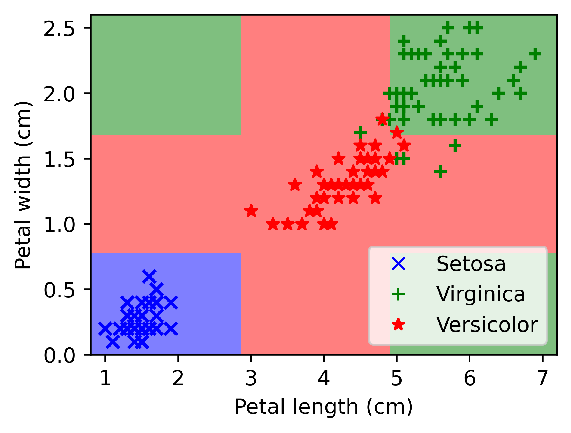
\includegraphics[width=0.20\linewidth]{figures/CLA/bb-knn.pdf}
			\label{fig:bb-knn}
		} &
		\subfloat[]{
			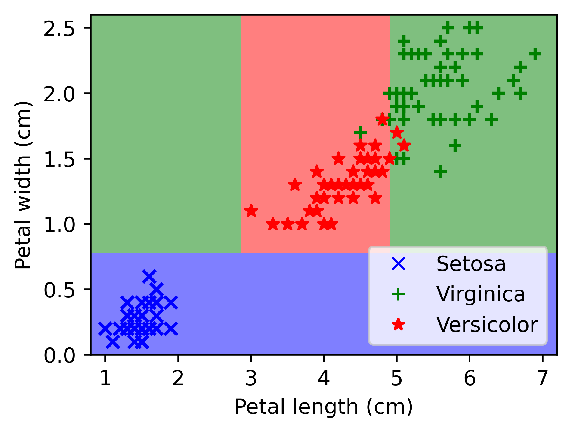
\includegraphics[width=0.20\linewidth]{figures/CLA/real-knn.pdf}
			\label{fig:real-knn}
		} &
		\subfloat[]{
			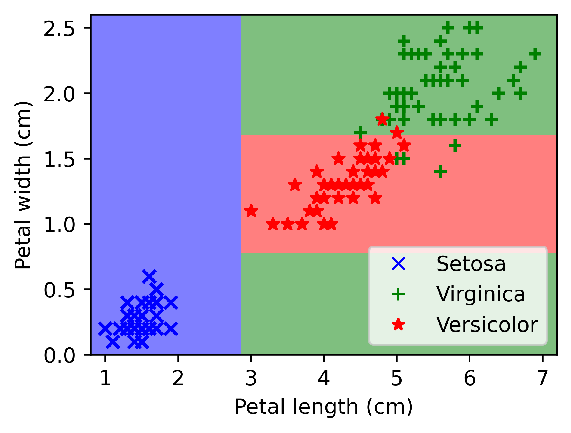
\includegraphics[width=0.20\linewidth]{figures/CLA/trepan-knn.pdf}
			\label{fig:trepan-knn}
		} &
		\subfloat[]{
			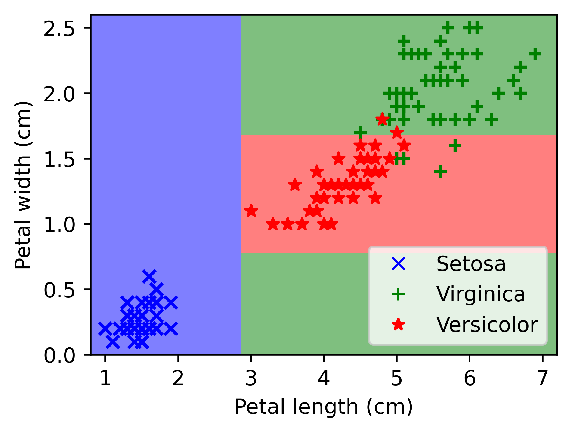
\includegraphics[width=0.20\linewidth]{figures/CLA/cart-knn.pdf}
			\label{fig:cart-knn}
		}
		\\
		\subfloat[MPL.]{
			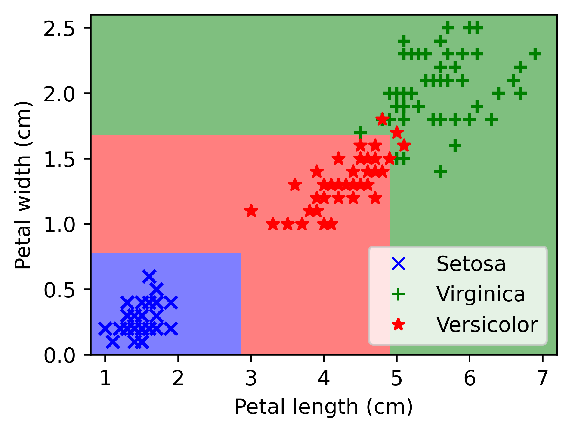
\includegraphics[width=0.20\linewidth]{figures/CLA/bb-mlp.pdf}
			\label{fig:bb-mlp-cla}
		} &
		\subfloat[]{
			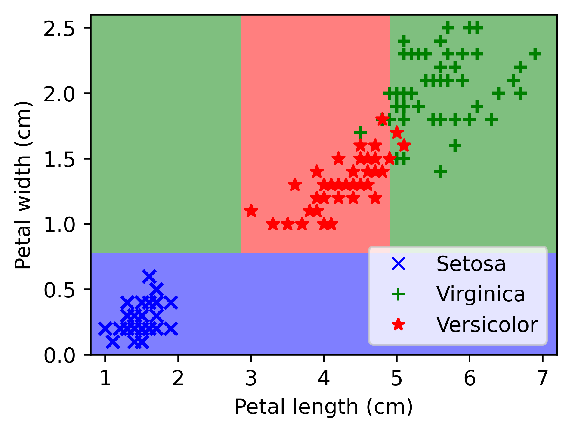
\includegraphics[width=0.20\linewidth]{figures/CLA/real-mlp.pdf}
			\label{fig:real-mlp}
		} &
		\subfloat[]{
			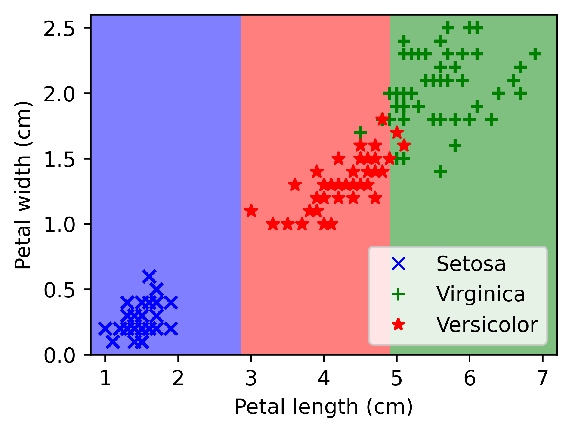
\includegraphics[width=0.20\linewidth]{figures/CLA/trepan-mlp.pdf}
			\label{fig:trepan-mlp}
		} &
		\subfloat[]{
			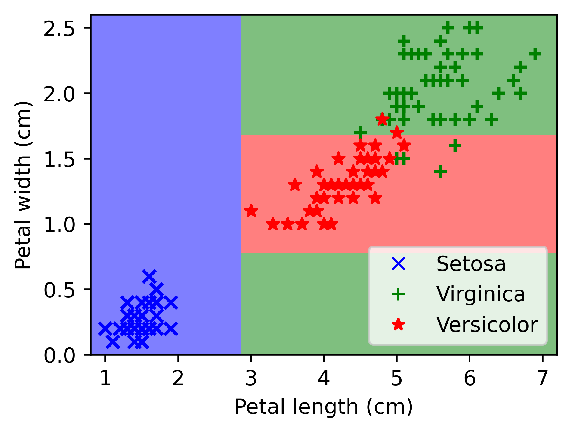
\includegraphics[width=0.20\linewidth]{figures/CLA/cart-mlp.pdf}
			\label{fig:cart-mlp-cla}
		}
		\\
		\subfloat[DT (binarised features).]{
			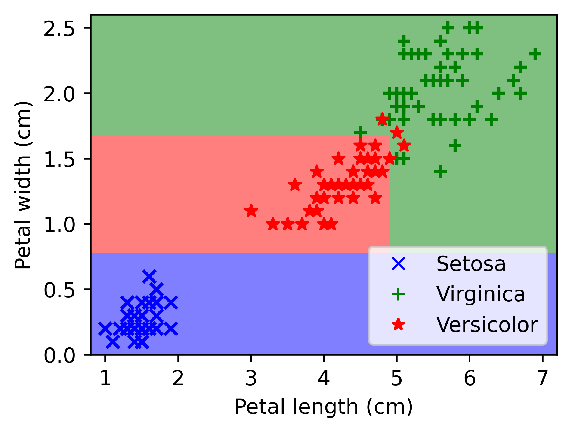
\includegraphics[width=0.20\linewidth]{figures/CLA/bb-dt.pdf}
			\label{fig:bb-dt-cla}
		} &
		\subfloat[]{
			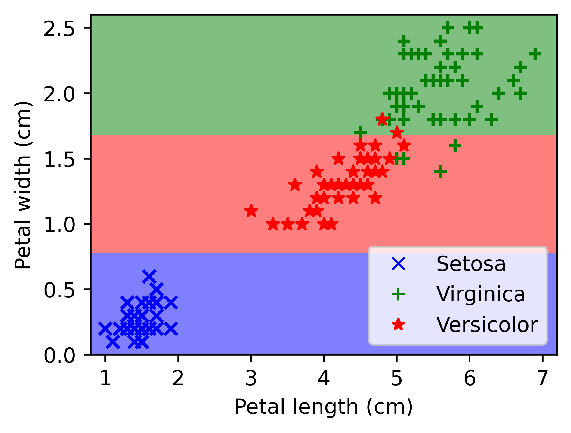
\includegraphics[width=0.20\linewidth]{figures/CLA/real-dt.pdf}
			\label{fig:real-dt}
		} &
		\subfloat[]{
			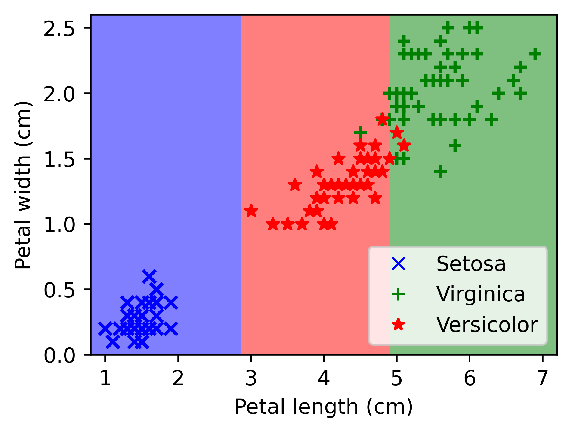
\includegraphics[width=0.20\linewidth]{figures/CLA/trepan-dt.pdf}
			\label{fig:trepan-dt}
		} &
		\subfloat[]{
			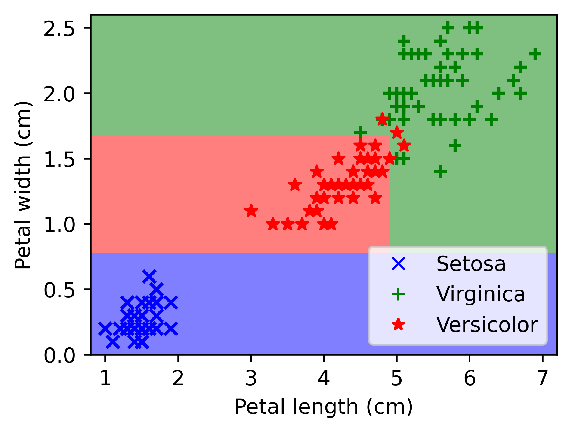
\includegraphics[width=0.21\linewidth]{figures/CLA/cart-dt.pdf}
			\label{fig:cart-dt-cla}
		}
		\\
		\subfloat[DT (continuous features).]{
			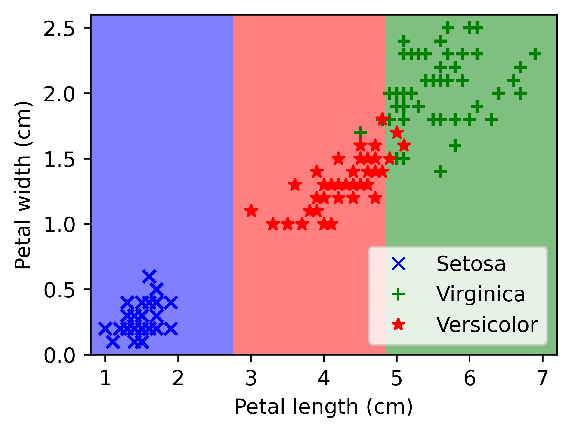
\includegraphics[width=0.21\linewidth]{figures/CLA/bb-dt-cont.pdf}
			\label{fig:bb-dt-cont}
		} & & &
		\subfloat[]{
			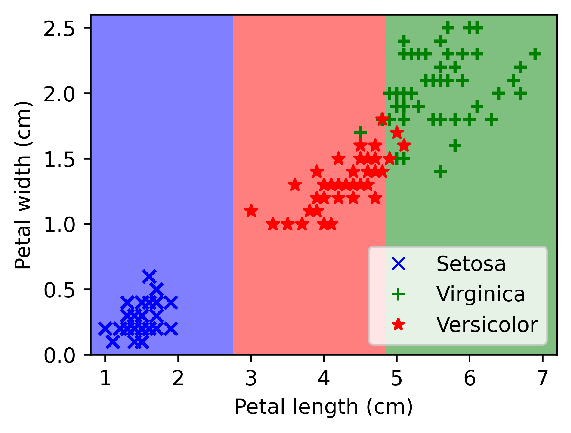
\includegraphics[width=0.21\linewidth]{figures/CLA/cart-dt-cont.pdf}
			\label{fig:cart-dt-cont}
		} \\
	\end{tabular}
	\caption[Comparison between Iris data set input space partitionings performed by the algorithms implemented in \psyke{}]{Comparison between Iris data set input space partitionings performed by the algorithms implemented in \psyke{}. Only the two most relevant features are reported---i.e., petal width and length. Missing subplots are due to the impossibility to apply \real{} and \trepan{} to BB classifiers trained with continuous input features}
	\label{fig:irisAll}
\end{figure}